\chapter{Les tests agiles}
\thispagestyle{fancy}
\section{ le testing agile et ses objectifs}
\label{sec:agiletest}
Avant l'agilité, les tests étaient souvent organisés de manière plus traditionnelle, en suivant un modèle de développement de logiciel en cascade. Les tests étaient généralement planifiés en fin de cycle de développement et étaient souvent considérés comme une étape de vérification plutôt qu'une activité intégrée au processus de développement. S'ajoute à cela le temps mort des testeurs pendant les phases de développememnt. Les tests étaient souvent effectués par une équipe distincte de testeurs et leur résultat était soumis à l'équipe de développement pour correction. Ce processus était souvent considéré comme inefficace et peu collaboratif.
\begin{center}
    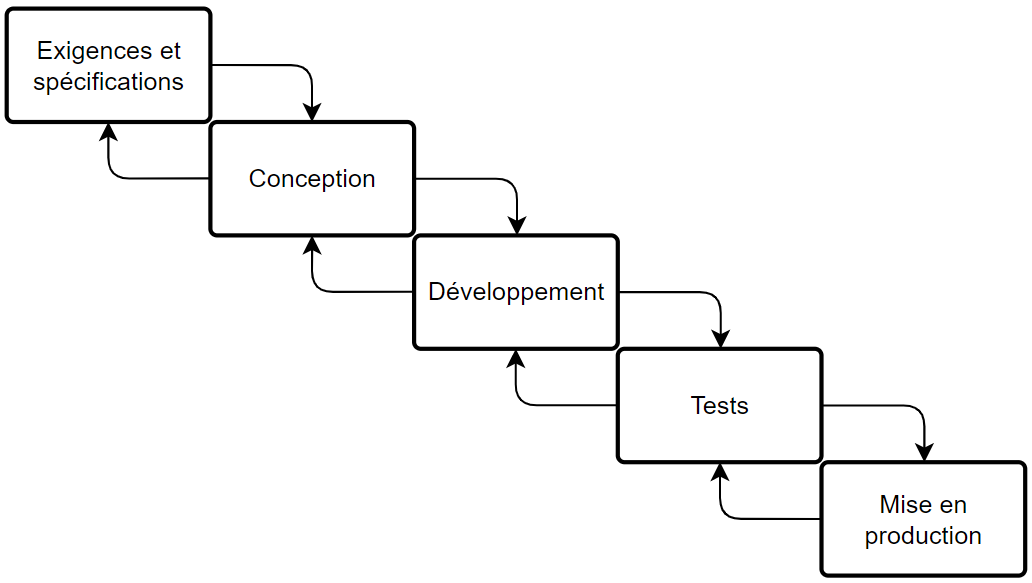
\includegraphics[width=0.7\textwidth]{incremental.png}
    % add description of the figure

    
\end{center}

\section{Le développement piloté par les tests}

TDD, BDD et ATDD sont trois approches différentes qui ont  apparues avec l'émérgence de l'agilité. Il consistent à développer des logiciels qui visent à garantir que le logiciel répond aux exigences et se comporte comme prévu en se basant sur des une planification des tests plus précoces dans le cycle de développement.

TDD : Un processus de développement de logiciels où les développeurs écrivent les tests en premier et écrivent ensuite du code pour faire passer les tests. L'accent est mis sur l'écriture de tests automatisés qui valident le comportement d'unités individuelles de code.

BDD : Une extension du TDD qui se concentre sur l'écriture de tests à un niveau d'abstraction plus élevé. Il vise à décrire le comportement du système du point de vue de l'utilisateur final, ce qui rend les tests plus lisibles et compréhensibles pour les parties prenantes qui ne sont pas familières avec le code \parencite{Bdd}.

ATDD : Semblable à BDD, l'ATDD est une approche de développement où les critères d'acceptation pour une histoire utilisateur sont définis avant le début du développement et des tests automatisés sont écrits pour valider que l'histoire a été correctement implémentée. L'accent est mis sur l'implication des parties prenantes dans le processus de test pour garantir que les exigences ont été correctement implémentées \parencite{AtddBook}.
\begin{center}
    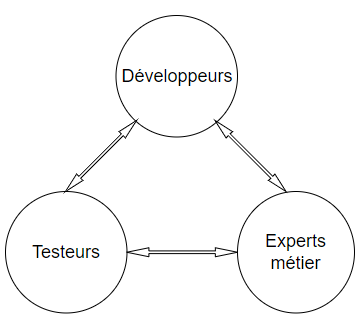
\includegraphics[width=0.5\textwidth]{interaction.png}
    \linebreak
fig:comment les choses doibe
\end{center}

Les scénarios BDD / ATDD sont souvent écrits en utilisant le format Gherkin "Given, When, Then", qui décompose le scénario en trois parties distinctes: "Given" quidécrit le contexte de départ de la situation, "When" décrit l'action qui déclenche le comportement à tester, et "Then" décrit les résultats attendus suite à l'action décrite dans "When". Ce format permet de clarifier les attentes du comportement du système, de fournir une documentation claire et concise des tests, et peut être utilisé en conjonction avec des outils de test automatisé pour automatiser les tests et faciliter le processus de développement logiciel.
\begin{center}
    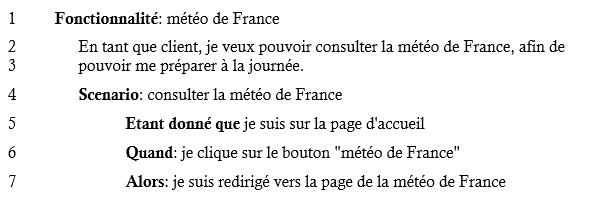
\includegraphics[width=0.7\textwidth]{feature.png}

\end{center}

\section{les contrainte des tests agiles}

\begin{itemize}
\item Coût élevé: 
la mise en place d'une infrastructure de test automatisé peut être coûteuse en termes de temps et de ressources.

\item Temps de développement prolongé: 
l'automatisation des tests peut prendre beaucoup de temps et peut ralentir le processus de développement.

\item Maintenance difficile: 
les tests automatisés peuvent nécessiter une maintenance constante pour s'assurer qu'ils restent pertinents et précis, ce qui peut être coûteux en temps et en ressources.
\item Difficulté à tester des scénarios complexes: 
il peut être difficile de tester des scénarios complexes avec des tests automatisés, ce qui peut entraîner une couverture insuffisante.
\item Dépendance de la qualité du code: 
la qualité des tests dépend directement de la qualité du code, donc si le code n'est pas correctement écrit, les tests peuvent ne pas être fiables.
\item Dépendance des compétences techniques: les tests automatisés nécessitent des compétences techniques pour les écrire et les maintenir, ce qui peut limiter leur utilisation dans certaines équipes.

\end{itemize}
Cependant, il convient de noter que ces inconvénients peuvent être minimisés en mettant en place une bonne stratégie de test et en choisissant les outils appropriés pour automatiser les tests. Les tests Agile peuvent également offrir de nombreux avantages, notamment une réduction des coûts, une amélioration de la qualité et une augmentation de la rapidité de déploiement.



